\documentclass[12pt, a4paper, titlepage]{article}

\setcounter{tocdepth}{3}

\usepackage{hyperref}
\usepackage{graphicx}
\usepackage{caption}
\usepackage{listings}
\usepackage{xcolor}
\lstset { %
  language=C++,
  backgroundcolor=\color{white}, % set backgroundcolor
  basicstyle=\footnotesize,% basic font setting
  breaklines=true,
  commentstyle=\color{red},
  frame=single,
  keepspaces=true,
  showstringspaces=false,
}
\usepackage{amsmath}

\title{SKFlatAnalyzer User Guide}
\author{Jae Sung Kim  \\
  Seoul National University \\
  jae.sung.kim@cern.ch
}
\date{\today} 

\begin{document}

\hypersetup{pageanchor=false}

\maketitle

\tableofcontents

\clearpage

\section{Introduction}

\subsection{SKFlat}
\begin{itemize}
\item A flat ntuple
\item Use MiniAOD as an input
\item GihHub link : \href{https://github.com/CMSSNU/SKFlatMaker}{https://github.com/CMSSNU/SKFlatMaker}
\item
  \begin{minipage}{\linewidth}
    \centering
    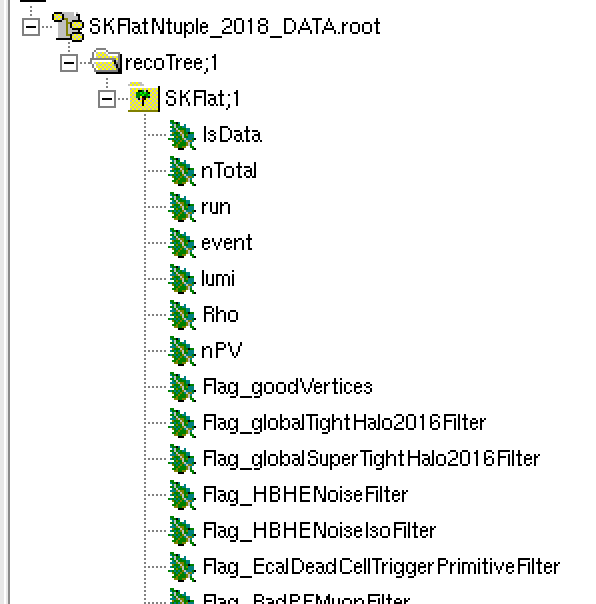
\includegraphics[width=10cm]{Figures/TreeContent.png}
  \end{minipage}
\end{itemize}

\subsection{SKFlatAnalyzer}
\begin{itemize}
\item ROOT6 based analyzer
\item SNU (tamsa1), KISTI and KNU batch are supported by same submission commands (2019.01.22)
\item Use SKFlat as an input
\item Run over each event, and do the analysis!!
\item Construct physics objects using branch elements
:
  \begin{lstlisting}
Muon mu;
double rc = muon_roch_sf->at(i);
double rc_err = muon_roch_sf_up->at(i);
mu.SetMiniAODPt(muon_pt->at(i));
mu.SetPtEtaPhiM(muon_pt->at(i)*rc, muon_eta->at(i), muon_phi->at(i), muon_mass->at(i));
  \end{lstlisting}
\item GitHub link : \href{https://github.com/CMSSNU/SKFlatAnalyzer}{https://github.com/CMSSNU/SKFlatAnalyzer}
\end{itemize}

\clearpage

\section{Directories}

\subsection{DataFormats/}

Physics objects

\subsection{Analyzers/}

Physics objects

\subsection{include/}

Header files

\subsection{src/}

Source files (define class, functions, ...)

\subsection{data/\$SKFlatV}

Various data files including .root, .txt, ...

E.g., fake rates, scale factors, …

Defined as an environment variable, \$DATA\_DIR

\subsection{python/}

Python scripts for job submission

\subsection{script/}

Any useful scripts

\subsection{lib/}

Compiled shared-libraries moved here

\clearpage

\section{Structure}

\subsection{Analyzer inheritance}

\begin{figure}[htbp]
\centering
  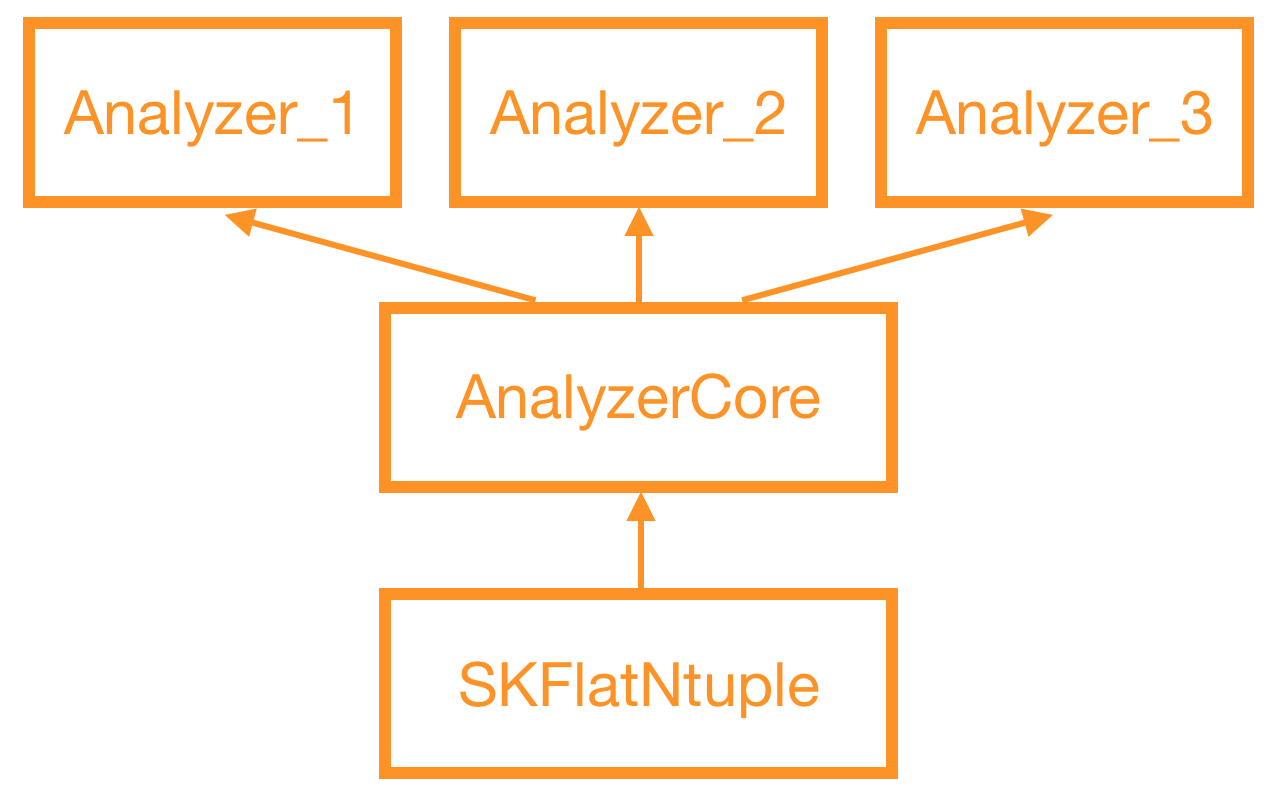
\includegraphics[width=1.0\textwidth]{Figures/AnalyzerInheritance.png}
  \caption{
    Diagram of analyzer inheritance.
  }
\end{figure}

\clearpage

\subsection{Physics object inheritance}

\begin{figure}[htbp]
\centering
  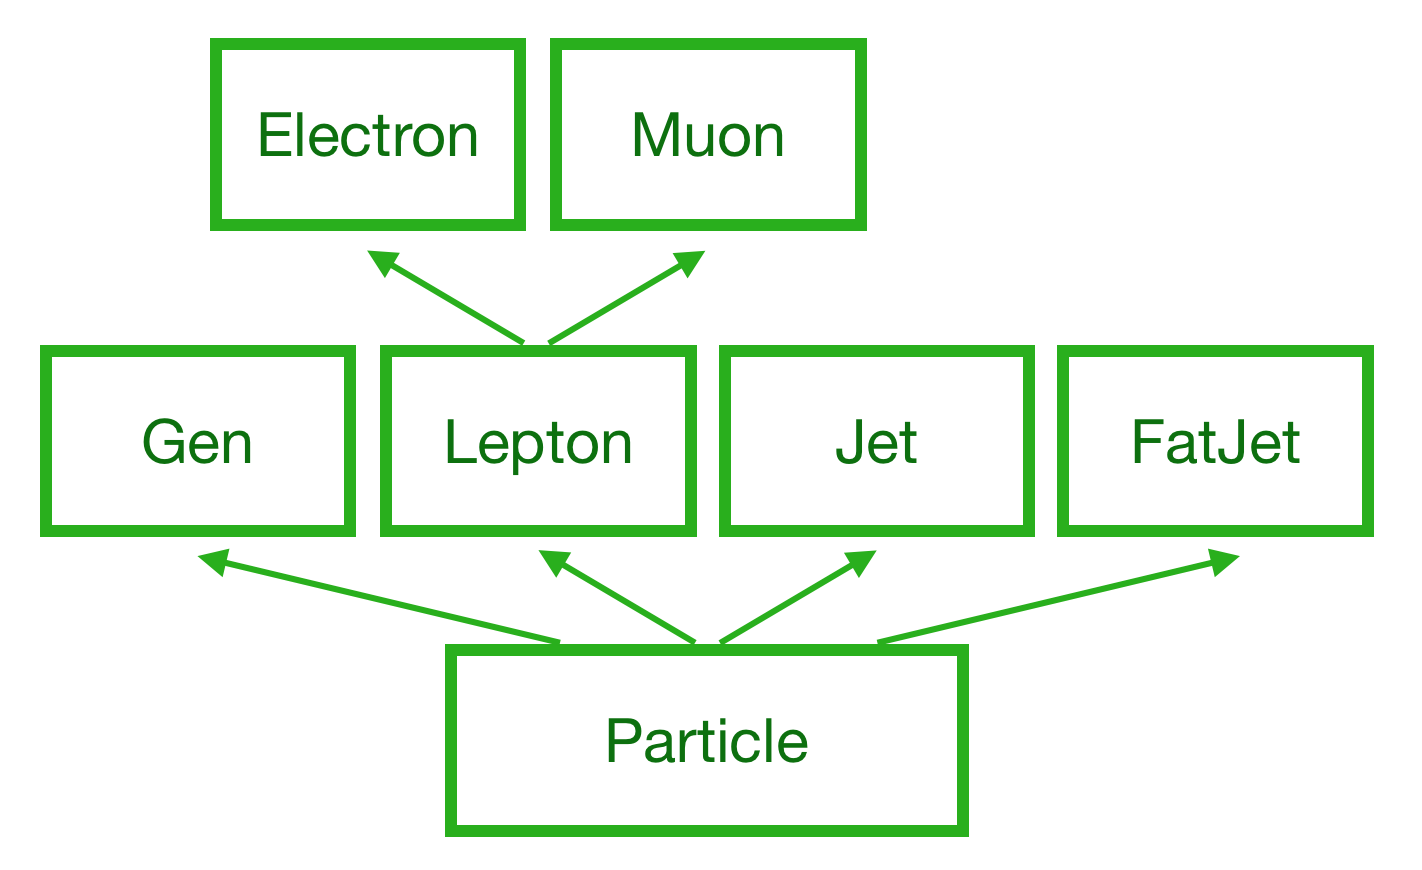
\includegraphics[width=1.0\textwidth]{Figures/PhysicsObjectInheritance.png}
  \caption{
    Diagram of physics object inheritance.
  }
\end{figure}

\clearpage

\section{Analyzer class and submission command}

\centerline{\textit{Every analyzer inherits AnalyzerCore}}
\centerline{\textit{AnalyzerCore inherits SKFlatNtuple}}

\subsection{SKFlatNtuple}

\begin{itemize}
\item Almost same as the output from TTree::MakeClass$()$
\item SKFlatNtuple::Loop$()$ loops over each event
%\item SKFlatNtuple::executeEvent$()$ is run for each event
%\item SKFlatNtuple::executeEvent$()$ is virtual. Define it in each Analyzer.
\end{itemize}

\subsection{AnalyzerCore}

\begin{itemize}
\item Inherits SKFlatNtuple
\item Includes header files of physics objects classes
\item Physics analysis functions
  \begin{lstlisting}
std::vector<Muon> AnalyzerCore::GetAllMuons(); // return all muons
std::vector<Muon> AnalyzerCore::GetMuons(TString id, double ptmin, double fetamax); // return muons passing ID selection
std::vector<Muon> AnalyzerCore::SelectMuons(std::vector<Muon> muons, TString id, double ptmin, double fetamax); // Select muons passing id out of pre-collected muon collections
  \end{lstlisting}
\item Histogram related functions
  \begin{lstlisting}
FillHist(TString histname, double value, double weight, int n_bin, double x_min, double x_max); // histogram is saved in the default directory of the output root file
JSFillHist(TString suffix, TString histname, double value, double weight, int n_bin, double x_min, double x_max); // histogram is saved in the directory named "suffix" of the output root file
  \end{lstlisting}
\item $($Example$)$
  \begin{lstlisting}
  vector<Electron> electrons = GetElectrons(param.Electron_Tight_ID, 10., 2.5);
  for(unsigned int i=0; i<electrons.size(); i++){

    Electron el = electrons.at(i);

    FillHist("RelIso", el.RelIso(), 1, 100, 0., 1.);
    JSFillHist(param.Electron_Tight_ID, "RelIso_"+param.Electron_Tight_ID, el.RelIso(), 1, 100, 0., 1.);

  }
  \end{lstlisting}
  \begin{minipage}{\linewidth}
    \centering
    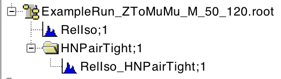
\includegraphics[width=10cm]{Figures/HistogramOutputExample.png}
  \end{minipage}
\item Even if two histograms are in different directories, if their names are the same, we have warning message : ``Warning in $<$TFile::Append$>$: Replacing existing TH1: RelIso $($Potential memory leak$)$."
\item So I recommend you to add directory name as a prefix/suffix of the histogram name : \par
Instead of ``RelIso" alone, use ``RelIso\_"+$<$Directory Name$>$
\end{itemize}

\subsection{MyAnalyzer}

\begin{itemize}
\item Inherits AnalyzeCore
\item Run by the job macro
\end{itemize}

\subsection{Job macro}

\begin{itemize}
\item Macro will be created \textit{automatically} by SKFlat$.$py command
\item MyAnalyzer object is declared
\item Input sample information $([$DATA$]$ DataStream $/$ $[$MC$]$ Sample name, input files, xsec, sumW$)$ is set
\item Output file path is set
\item SKFlatNtuple::Init$()$ is run :
Initializing branch element variables
\item AnalyzerCore::initializeAnalyzer$()$ is run
\begin{itemize}
\item This function is virtual, and can be redefined in ExampleRun
\item Anything you want to do before the event loop can be done here
\item Userflag is supported by python$/$SKFlat$.$py, by the option \par ``$--$userflags flag1,flag2,flag3"
\item The existence of a flag can be checked by using \par AnalyzerCore::HasFlag$($TString flag$)$
\end{itemize}
\item SKFlatNtuple::Loop$()$ is run : loop over events
\item AnalyzerCore::WriteHist$()$ is run : write histograms in the output
\end{itemize}

\subsection{SKFlat.py}

Script for batch job submission

\subsection{Simple way for debugging}

When debugging, it is better use the master node rather than using batch system.
Here is a quick intstruction to create a debugging macro script.

Let's say you want to debug `MyAnalzyer'.
Then, run (-n 10 can be any number) : \\
\centerline{SKFlayt.py -a MyAnalzyer -n 10 -i $<$sample$>$ -y $<$year$>$ $--$no\_exec}
Go to the job directory. It should be : \\
\$SKFlatRunlogDir/$<$MyAnalzyer\_\_$<$TIMESTAMP$>$\_\_Year$<$year$>$\_\_$<$sample$>$\_\_$<$machine$>$
If in KISTI, you will have run\_XYZ.C's.
If in SNU or KNU, you will have job\_XYZ/run.C's.
Copy one of them (let's call it as ``run.C") to \$SKFlat\_WD.
If SNU or KNU, edit the path for libDataFormats.so and libAnalyzers.so as follows;
\begin{lstlisting}
R__LOAD_LIBRARY(./lib/libDataFormats.so)
R__LOAD_LIBRARY(./lib/libAnalyzers.so)
\end{lstlisting}
Now, ``run.C" uses the libraries in \$SKFlat\_WD/lib, which is updated when you run ``make".
So, edit your codes, compile, and then do ``root -l -b -q run.C" in \$SKFlat\_WD.

Here are some useful lines you can add in ``run.C" :
\begin{itemize}
\item ``m.MaxEvent $=$ 1000;" : run 1000 events only
\item ``m.NSkipEvent $=$ 10;" : skip first 10 events, and then run ``m.MaxEvent" events. If ``m.MaxEvent" is not set, run to the end.
\item ``m.LogEvery $=$ 2" : print current event number for every 2 events.
\end{itemize}

\clearpage

\section{Macro run order}

\subsection{Example of a macro with comments inline}

\begin{lstlisting}
R__LOAD_LIBRARY(libPhysics.so)
R__LOAD_LIBRARY(libTree.so)
R__LOAD_LIBRARY(libHist.so)
R__LOAD_LIBRARY(./lib/libDataFormats.so)
R__LOAD_LIBRARY(./lib/libAnalyzers.so)

void run(){

  //==== Declaring an analyzer class immediately runs followings in orders; 
  //==== 1) Constructor of SKFlatNtuple is called
  //==== 2) Constructor of AnalyzerCore is called
  //==== 3) Constructor of ExampleRun is called
  ExampleRun m;

  //==== SKFlat ntuple directory structure..
  m.SetTreeName("recoTree/SKFlat");

  //==== DATA or MC?
  m.IsDATA = true;
  //==== If DATA, PD name
  m.DataStream = "SingleMuon";
  //==== DATA year
  m.DataYear = 2016;
  //==== Files to be ran with this macro
  m.AddFile("SKFlatNtuple_2016_DATA_100.root");
  //==== output rootfile path
  m.SetOutfilePath("hists.root");
  //==== SKFlatNtuple::Init(), which does SetBranchAddress()
  m.Init(); 
  //==== AnalyzerCore::initializeAnalyzerTools Read histograms or initialize MCCorrection helpers or data-driven estimators
  m.initializeAnalyzerTools();
  //==== Any initialization just before running event loop. This is only ran once within a macro. For example, you should run AnalyzerCore::HasFlag() here. More example can be found HERE
  m.initializeAnalyzer();
  //==== Finally, run event loops
  m.Loop();

  //==== All events are ran. Now write histograms to the output rootfile
  m.WriteHist();
}

\end{lstlisting}

\clearpage

\section{Migration from CATAnalyzer}

Direct copy from CATAnalyzer codes to SKFlatAnalyzer won't work, but here are some tips.

\begin{itemize}

\item FillHist$($histname, variable, weight, x\_min, x\_max, n\_bin) \par
      $\rightarrow$ FillHist$($histname, variable, weight, n\_bin, x\_min, x\_max) \par
      : follow the order of arguments of TH1 in ROOT

\end{itemize}

\clearpage

\section{Rules for developers}

Some rules you should follow, if you want to make a pull request to the master branch.

\subsection{File/Function/Variable names are important}

Let's spend enough time for naming our new file/function/variable...
Good naming makes programming efficient.

\subsection{Equality operator between float or double}

Guess what you would get from ``root -l -b -q test.C" with below.

\begin{lstlisting}
float GetFatJetSF(float tau21cut){
  
  if(tau21cut == 0.45){
    return 0.45;
  }
  if(tau21cut == 0.6){
    return 0.6;
  }
  else{
    return 1.;
  }

}

void test(){

  cout << "Value : " << GetFatJetSF(0.45) << endl;

}

\end{lstlisting}

Result is \textbf{Value : 1}.
It works properly if you change \textbf{float GetFatJetSF(float tau21cut)} to \textbf{float GetFatJetSF(double tau21cut)}.
However, it is NOT recommended to apply equality operator between floats.
If you really need it, you can do $|A-B|<e$ with a very small $e$ $($e.g., 0.001$)$.

\subsection{std::map is good, but be careful}

We use a lot of std::map in the analyzer; rootfile for MCCorrection are saved as ``std::map$<$TString, TH1D$>$ histmap",
and histogram can be accessed by ``histmap$[$key$]$".
But if you store so many histograms into the map, it spends so much time to obtain ``histmap$[$mykey$]$",
because it checks ``mykey==key" for each keys.
If you have saved thousands of fake-rate histograms into a map and run a fake estimation, it will take years...
If you are applying muon scale factors,
``map\_hist\_Muon$[$YOUR\_ID$]$" is ran for each event and each muons.
If you wrote too many IDs in ID/Muon/histmap.txt, you will waste your time looping over unnecessary keys.
To save your time, you can add a ``\#" at the beginning of each lines in ``\href{https://github.com/CMSSNU/SKFlatAnalyzer/blob/Run2Legacy\_v1\_\_190123/data/Run2Legacy\_v1/2016/ID/Muon/histmap.txt}{ID/Muon/histmap.txt}" (i.e., deactivating it) : \\
\centerline{ID SF NUM\_MediumID\_DEN\_genTracks RunAveraged\_SF\_ID.root NUM\_MediumID\_DEN\_genTracks\_eta\_pt}
\centerline{$\downarrow$}
\centerline{\#ID SF NUM\_MediumID\_DEN\_genTracks RunAveraged\_SF\_ID.root NUM\_MediumID\_DEN\_genTracks\_eta\_pt}
Then histogram for Medium ID will not be saved in the histmap.

\subsection{When using random variables..}

Some functions use random variables (e.g., smearing from a distribution).
If you use default random seed, your results can be changed everytime you run the analyzer.
Easiest way to avoid this issue is using a combination of RunNumber and EventNumber as a seed.
E.g., $\text{seed} = \text{RunNumber} \times 1000000000 + \text{EventNumber}$.

\end{document}
